% 图 24.1 —— 由 `checks/emit_hand.py` 自动拼出（probe 精测 + prims2 图元分解）
%%
% ⚠ 这是**稿子不是成品**：跑 `checks/checkhand.py 24.1` 看指标 + 看叠合图。
%%
%% ⚠ 待核：
%   · 本图 probe 报出阴影族 1 个 —— **本脚本不生成阴影**（要照原书手写）；prims2 的 strokes 里可能含阴影线，核对时留意别画重
%   · 可疑字形 1 项（空心圈 ⊙ 常被认成字母 o）—— 见文件末
%%
\documentclass[12pt]{standalone}
\usepackage{fontspec}
\setsansfont{Arial}
\newfontfamily\mfallback{DejaVu Sans}
\usepackage{tikz}
\usetikzlibrary{arrows.meta}
\begin{document}
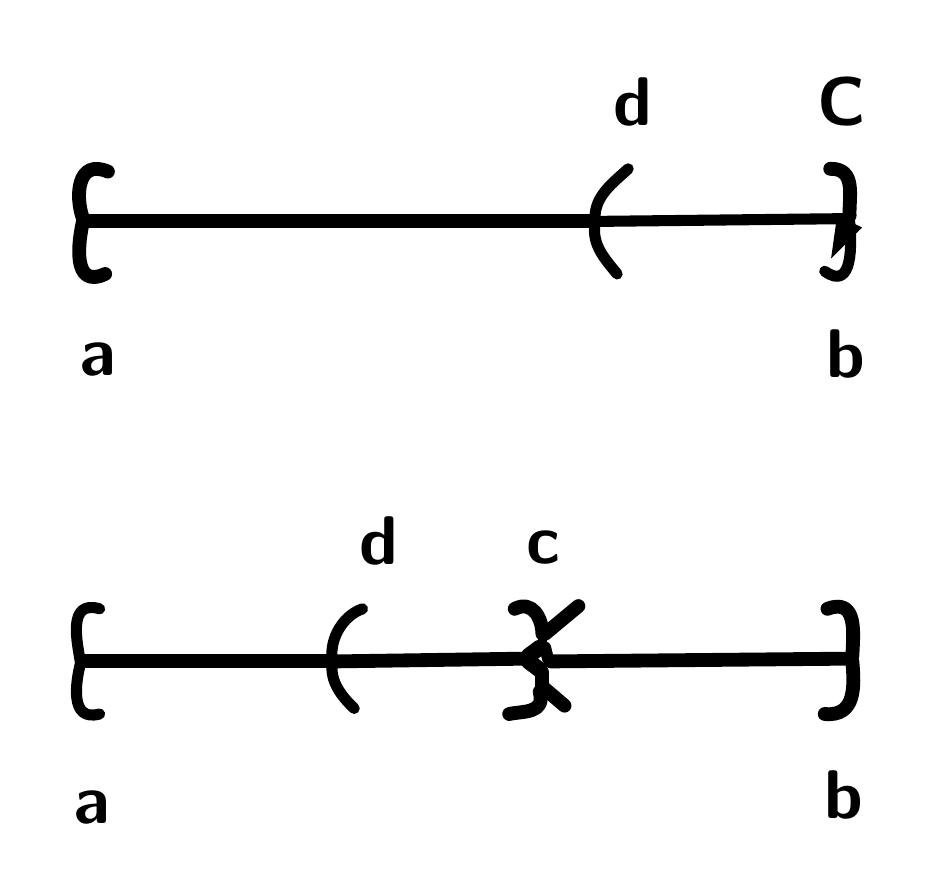
\begin{tikzpicture}[x=1pt, y=-1pt, line width=5.0pt, line cap=round, line join=round]

  %% ════ 填充区（prims2 的 fills）════

  %% ════ 直线段（prims2 的 strokes）════
  \draw[line width=5.0pt] (109.0,229.0) -- (20.0,229.0);
  \draw[line width=5.0pt] (180.0,228.0) -- (111.0,229.0);
  \draw[line width=5.0pt] (21.0,70.0) -- (204.0,70.0);
  \draw[line width=5.7pt] (181.0,227.0) -- (185.0,224.0);
  \draw[line width=4.0pt] (296.0,69.0) -- (206.0,70.0);
  \draw[line width=3.0pt] (186.0,223.0) -- (186.0,220.0);
  \draw[line width=5.7pt] (181.0,229.0) -- (185.0,232.0);
  \draw[line width=4.3pt] (188.0,228.0) -- (187.0,224.0);
  \draw[line width=5.0pt] (199.0,209.0) -- (187.0,219.0);
  \draw[line width=5.0pt] (186.0,238.0) -- (186.0,233.0);
  \draw[line width=5.0pt] (194.0,245.0) -- (187.0,239.0);
  \draw[line width=5.0pt] (297.0,228.0) -- (189.0,229.0);

  %% ════ 曲线（prims2 的 curves —— 三段式，坐标同为 (y,x)）════
  \draw[line width=5.0pt] (185.0,240.0) .. controls (187.3,248.0) and (178.8,246.9) .. (174.0,248.0);
  \draw[line width=4.0pt] (19.0,230.0) .. controls (17.5,236.1) and (14.9,251.0) .. (26.0,248.0);
  \draw[line width=4.0pt] (110.0,228.0) .. controls (109.2,220.5) and (114.0,212.4) .. (121.0,210.0);
  \draw[line width=5.0pt] (298.0,229.0) .. controls (298.7,237.6) and (299.5,249.1) .. (288.0,248.0);
  \draw[line width=5.0pt] (28.0,89.0) .. controls (15.8,94.7) and (18.4,76.8) .. (20.0,70.0);
  \draw[line width=4.0pt] (205.0,69.0) .. controls (204.8,60.8) and (211.5,56.1) .. (217.0,51.0);
  \draw[line width=5.0pt] (186.0,219.0) .. controls (185.9,213.4) and (182.4,206.7) .. (176.0,210.0);
  \draw[line width=4.0pt] (110.0,230.0) .. controls (109.4,236.5) and (113.4,241.6) .. (118.0,246.0);
  \draw[line width=4.0pt] (205.0,71.0) .. controls (203.8,78.5) and (208.7,83.7) .. (213.0,89.0);
  \draw[line width=5.0pt] (290.0,51.0) .. controls (299.6,50.8) and (296.7,61.2) .. (297.0,68.0);
  \draw[line width=4.0pt] (288.0,88.0) .. controls (298.5,95.6) and (297.7,77.7) .. (297.0,70.0);
  \fill (292.5,67.8) -- (301.5,72.2) -- (290.3,83.4) -- cycle;
  \draw[line width=4.0pt] (19.0,229.0) .. controls (18.0,222.5) and (14.1,206.5) .. (26.0,210.0);
  \draw[line width=5.0pt] (289.0,210.0) .. controls (300.1,205.8) and (298.3,219.2) .. (298.0,227.0);
  \draw[line width=5.0pt] (29.0,52.0) .. controls (17.8,47.2) and (17.1,61.2) .. (20.0,69.0);

  %% ════ 实心点 ════
  % （略）(300.5,69.5) r=6.5 落在箭头头上 —— 已由箭头头代替

  %% ════ 标签（probe 直接给的 \node 行）════
  %% ⚠ 全部补了 fill=white：文字在最上层，否则与曲线交叉干扰
     \node[anchor=center,inner sep=0pt,fill=white,font=\fontsize{31.5}{39.4}\selectfont] at (218.8,26.8) {\textsf{\textbf{\textit{d}}}};   % box(208,14,19,23)
     \node[anchor=center,inner sep=0pt,fill=white,font=\fontsize{23.4}{29.3}\selectfont] at (294.1,26.7) {\textsf{\textbf{\textit{C}}}};   % box(286,18,15,17)
     \node[anchor=center,inner sep=0pt,fill=white,font=\fontsize{30.7}{38.3}\selectfont] at (295.8,117.8) {\textsf{\textbf{\textit{b}}}};   % box(286,105,17,23)
     \node[anchor=center,inner sep=0pt,fill=white,font=\fontsize{31.0}{38.7}\selectfont] at (25.5,120.0) {\textsf{\textbf{\textit{a}}}};   % box(17,110,15,17)
     \node[anchor=center,inner sep=0pt,fill=white,font=\fontsize{30.8}{38.5}\selectfont] at (126.8,185.3) {\textsf{\textbf{\textit{d}}}};   % box(116,173,19,22)
     \node[anchor=center,inner sep=0pt,fill=white,font=\fontsize{30.5}{38.1}\selectfont] at (186.3,188.0) {\textsf{\textbf{\textit{c}}}};   % box(178,178,15,17)
     \node[anchor=center,inner sep=0pt,fill=white,font=\fontsize{30.0}{37.5}\selectfont] at (294.8,277.2) {\textsf{\textbf{\textit{b}}}};   % box(285,265,17,22)
     \node[anchor=center,inner sep=0pt,fill=white,font=\fontsize{31.0}{38.7}\selectfont] at (23.5,282.0) {\textsf{\textbf{\textit{a}}}};   % box(15,272,15,17)

  % 钉死画布：否则超出的图元/控制点会把页面撑大，1:1 回比就失准
  \pgfresetboundingbox
  \path[use as bounding box] (0,0) rectangle (314,296);
\end{tikzpicture}
\end{document}

% ⚠ 待核清单（probe 拿不准，人眼过一遍）：
%   · 未识别/跳过：⑤ 跳过/未识别的字形
